\documentclass{report}

\usepackage[margin=1in]{geometry}
\usepackage{amsmath,amssymb}
%\usepackage{dsfont} %install texlive-fonts-extra 
\usepackage{tikz}
\usetikzlibrary{bayesnet}
\usepackage{setspace}
\usepackage{xcolor}
\usepackage[toc,page]{appendix}

\author{Otto Fabius}
\title{SGVB Topic Modeling}
\newcommand{\specialcell}[2][c]{%
	\begin{tabular}[#1]{@{}l@{}}#2\end{tabular}}
\begin{document}
\large
\doublespacing
\maketitle

\begin{abstract}
	content...
\end{abstract}
\chapter*{}
\onehalfspacing
\section*{List of Symbols}
We use lowercase bold-faced symbols to denote vectors, and uppercase bold-faced symbols to denote matrices. \\ \\
\begin{tabular}{r l}
	\hspace{15mm} $\mathbf{x}$ & Data point \\
	$\mathbf{\hat{x}}$ & Data point normalized to have unit length \\	
	$\theta$ &  Model parameters \\
	$\phi$ & Parameters of approximate posterior model \\
	$z$ & Stochastic latent variable\\
	$\mu$ & Mean of stochastic latent variable\\
	$\sigma ^2 $ & Variance of stochastic latent variable \\
	$\mathcal{L}$ & Lower Bound \\
	$\tilde{\mathcal{L}}$ & Lower Bound estimate\\
	$\tilde{\mathcal{L}_w}$ & Per-word lower bound estimate \\
	$D_{KL}$ & Kullback-Leibler Divergence \\
	$V$ & Number of unique words in a dataset. \\
	$N_d$ & Number of documents in a dataset. \\
	$F$ & Matrix of node feature vectors
\end{tabular}
\\ \\
 We use index $i$ to indicate a data point, index $k$ to indicate a feature, and index $j$ to indicate a latent variable. In all applications in this thesis, our data points are documents represented by count vectors. Therefore, for example, $\mathbf{\hat{x}}_{ik}$ is the relative frequency of word $k$ in document $i$.
\section*{List of Abbreviations}
\begin{tabular}{r l}
	\hspace{10mm} BoW & Bag-of-Words \\
	DEF & Deep Exponential Families \\
	GCE & Graph Convolutional Encoder \\
	LDA & Latent Dirichlet Allocation \\
	SGVB & Stochastic Gradient Variational Bayes \\
	VAE & Variational Autoencoder \\
\end{tabular}

\tableofcontents

\doublespacing
\chapter{Introduction}
Aim, scope and structure of the thesis. 
\section{Research question}
Explain that we want to use sgvb for topic modelling. Introduce research question:
Can we perform large-scale, efficient, high-quality inference on bag-of-words representations of documents with sgvb? \\
Briefly discuss the advantages of this approach compared to other methods in topic modelling (one paragraph)
-	How do we deal with large vocabulary size?\\
-	What consequences do sparsity have/how can they be overcome? \\
-	What is learned in the (continuous) latent representation?



\pagebreak 
\nocite{*}
\bibliographystyle{amsplain}

\chapter{Background}
\section{Variational Inference}
\begin{itemize}
	\item Variational Optimization key idea
	\item Often used for inference problems, decompose the log marginal according to Bishop (eq 10.2)
	\item 
\end{itemize}
Variational Inference methods in general are used when data $\mathbf{X}$ is assumed to be generated through some process from an underlying set of stochastic latent variables $\mathbf{Z}$. The probability of data is therefore modeled as $p(\mathbf{X}) = p(\mathbf{Z}|\mathbf{X})p(\mathbf{Z})$. Moreover, this set of methods is used when the true posterior $p(Z|X)$ can not be evaluated analytically. Variational Bayes introduces a tractable distribution $q(\mathbf{\mathbf{Z}|\mathbf{X}})$ as an approximation to $p(\mathbf{Z}|\mathbf{X}))$.
\\
More on Variational Inference....
\section{Bag-of-words Topic Modelling}

\subsection{LSI and pLSI}
\subsection{LDA}
Explain LDA following (p)LSI and Variational Inference.
\subsection{Deep Exponential Families}

Deep exponential families is relevant for this work for two reasons: It shows that deeper models can be more powerful than LDA, and is currently the state of the art. Nothing in our methods depends on this section.


\section{SGVB}\label{sgvb_section}

Discuss requirements of problem scenario for SGVB to be applicable. \\

Notes:\\
- No simplifying assumptions are made about the marginal or posterior probabilities, as is the case in other VB methods (check!!) \\
- $q(\mathbf{Z}|\mathbf{X})$ is not necessarily factorial and its parameters $\phi$ are not computed from some closed-form expectation (as in mean field VI)
- General purpose introduction of sgvb . \\

- areas of success of sgvb.

- compare VAE to LDA:

\subsection{Relation to LDA}

Discuss how closely related Graphical models are. Note that sampling separately for each word could facilitate the extra plate LDA has in a VAE approach, but then not only inefficient but also not possible to learn non-linear dependencies between words.

\begin{figure}\label{LDAVAE GM}
	\centering
	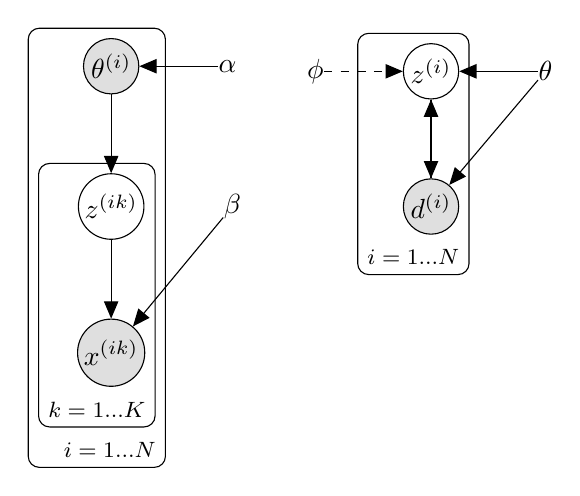
\begin{tikzpicture}[node distance = 1.5cm]
	\node[obs] (x) {$x^{(ik)}$}; 
	
	\node[latent, above=of x] (z) {$z^{(ik)}$}; 
	
	\node[obs, above=of z] (d) {$\theta^{(i)}$}; 
	
	\node[const, right=of d] (a) {$\alpha$} ;
	\node[const, right=of z] (th) {$\beta$} ;
	
	\edge {a} {d};
	\edge {z} {x};
	\edge {d} {z};
	\edge {th} {x};
	
	
	\plate {xz} {(x)(z)} {$k = 1...K$};
	\plate {xzd} {(x)(z)(d)(xz)} {$i = 1...N$};
	
	
	
	\node[const, right=of th] (extra) {};
	\node[obs, right=of extra] (d2) {$d^{(i)}$};
	
	\node[latent, above=of d2] (z2) {$z^{(i)}$};
	
	\node[const, right=of z2] (th2) {$\theta$} ;
	\node[const, left=of z2] (ph2) {$\phi$};
	
	
	\edge {z2} {d2};
	\edge {th2} {z2};
	\edge {th2} {d2};
	\edge [dashed,bend left] {d2} {z2}
	\edge [dashed] {ph2} {z2}
	
	
	
	\plate {zd2} {(z2)(d2)} {$i = 1...N$};
	
	
	\end{tikzpicture}
	\caption{Graphical Model of LDA (left) and VAE Topic Model (left)}
\end{figure}

\subsection{Neural Variational Inference for Topic Models}

\section{Stick-Breaking VAE}\label{sbvae_section}
	As detailed in \ref{sgvb_section}, one restriction of SGVB in general is the need for a differentiable, non-centered parametrization of the latent variables. Therefore, e.g. Beta distributed latent variables (as used in e.g. LDA \cite{bleil2003latent}), can not be used in the SGVB framework. \\ Nalisnyck \& Smith extend SGVB to Stick-breaking priors by using the Kumaraswami Distribution as the approximate posterior. The rest of this section \ref{sbvae_section} is not much more than a description of the relevant part of Nalisnyck \& Smyth \cite{nalisnick2016deep}.
	
	
	\subsection{The Stick-Breaking Process}\label{sb_process}
	
	\subsection{The Kumaraswami Distribution}\label{kum}
	

\chapter{SGVB Topic Models}
In this Chapter, we present in detail the models and methods we use in our experiments. 

\section{Topic VAE}\label{TopicVAE}

In this section we describe our initial approach for topic modeling with SGVB. It closely resembles the VAE model used in the experiments by Kingma and Welling\cite{kingma2013auto}, so one might call this a Topic VAE. We will describe the application-specific choices made within the general SGVB framework as described in section \ref{sgvb_section}, and derive the objective function used for optimization. 

\subsection{Model Specifics}

Within the general SGVB framework described in the previous chapter, we specify the following characteristics of our VAE Topic model:

\begin{enumerate}
	\item The representation of our documents $\mathbf{X}$
	\item The encoder $q(\mathbf{z}|\mathbf{x})$
	\item $p(z)$, a prior  over the latent variables
	\item A differentiable way of sampling $\mathbf{z}$ from $p(\mathbf{z}|\mathbf{x})$. 
	\item The decoder $p(\mathbf{x}|\mathbf{z})$
\end{enumerate}

The representation of the documents is a normalized Bag-of-Words representation s.t. document $i$ is represented by a unit vector $\hat{\mathbf{x}_i} = \frac{\mathbf{x}_i}{\sum_{k=1}^{V}x_{ik}}$. Although normalizing data is standard practice in neural network approaches (e.g. \cite{bishop1995neural}), typically each feature is normalized independently to have zero mean and unit variance. In our approach, however, all features (word counts) of a data point (document) are normalized s.t. they represent word probabilities.  Note that this representation no longer contains information on the length of documents, so this approach assumes the latent representations are independent of document length.
\\
The encoder $q(\mathbf{z}|\mathbf{x})$ is a fully connected neural network with one or more hidden layers with ReLu activation functions. The input is $\mathbf{d}$ and the output is the mean and log standard deviation \{$\boldsymbol{\mu}, \log \boldsymbol{\sigma} ^2\}$ of the Multivariate Gaussian $N(\boldsymbol{\mu}, \boldsymbol{\sigma} ^2\textbf{I})$. For one hidden layer this would be the following function:
\begin{align}
\mathbf{h_{e1}} = \text{ReLu}(\mathbf{\hat{x}}\mathbf{W_{e1}} + \mathbf{b}) \label{he1}\\
\boldsymbol{\mu} = \mathbf{h_{e1}W}_{\mu} \label{vae_encoding_mu} \\
\log \boldsymbol{\sigma}^2 = \mathbf{h_{e1}W}_{\sigma} \label{vae_encoding_sig}
\end{align} 


Our encoder therefore only differs from the encoder used in the experiments in Kingma \& Welling \cite{kingma2013auto} because we use the ReLU function and, in some cases, multiple hidden layers. We also use the same prior over latent variables, $p(\mathbf{z}) = N(0,\textbf{I})$ and the same (differentiable) sampling method as in \cite{kingma2013auto}: we use transformation function $g_\phi(\boldsymbol{\epsilon},\mathbf{x}) = \boldsymbol{\mu} + \boldsymbol{\sigma}^2\odot \boldsymbol{\epsilon}$, and sampling function $p(\epsilon) = N(0,\textbf{I})$. \\
The decoder $p(\mathbf{x}|\mathbf{z})$ is also a neural network with as input (a sample from) latent representation $\mathbf{z}$ and as output the probabilities of a Multinomial distribution, with a ReLu activation function used in each hidden layer. With one hidden layer, this would specified by:

\begin{align}
\mathbf{h_{d1}} = \text{ReLu}(\mathbf{zW_{d1}+b_{d1}})
\\
p(\mathbf{x}|\mathbf{z}) = \text{softmax} (\mathbf{h_{d1}W_{d2}}+\mathbf{b_{d2}})
\end{align}
Where the $\text{softmax}(\mathbf{x}) = \dfrac{e^{\mathbf{x}}}{\sum_{k=1}^{K}e^{x_k}}$



Discuss alternative approach with separate latent variables and/or noise for each word?\\ \\

\subsection{Objective Function}
The general form of the SGVB estimator is:

\begin{align}
\tilde{\mathcal{L}}(\boldsymbol{\theta}, \boldsymbol{\phi}, \mathbf{x_i}) = -D_{KL}(q_\phi (\mathbf{z}|\mathbf{x}_i)||p_\theta(\mathbf{z}))  + \frac{1}{L}\sum_{l=1}^{L}\log p_\theta(\mathbf{x}_i|\mathbf{z}_i^{(l)})
\end{align}

And because we consistently only use one sample from $p(\boldsymbol{\epsilon})$ per data point, this simplifies to:

\begin{align}\label{lb_summary}
\tilde{\mathcal{L}}(\boldsymbol{\theta}, \boldsymbol{\phi}, \mathbf{x_i}) = -D_{KL}(q_\phi (\mathbf{z}|\mathbf{x}_i)||p(_\theta(\mathbf{z}))  + \log p_\theta(\mathbf{x}_i|\mathbf{z}_i)
\end{align}

Because we use Gaussian latent variables with diagonal covariance, we can integrate the KL Divergence analytically as done in Kingma and Welling \cite{kingma2013auto}. \textit{Might need to elaborate on this, if not already done so in the background chapter}. Adding the expression for the Multinomial likelihood $p_\theta(\mathbf{x}_i|\mathbf{z}_i)$, we then have
\begin{align}\label{LBest}
\tilde{\mathcal{L}}(\boldsymbol{\theta}, \boldsymbol{\phi}, \mathbf{x_i}) = - \frac{1}{2}\sum\limits_{j=1}^{J}\{1+\log \sigma_{\phi ,ij}^2 - \mu_{\phi,ij}^2 - \sigma_{\phi ,ij}^2\}  + 
\sum_{k=1}^K x_{ik} \log (y_{ik})
\end{align}
\\
Notably, this is the lower bound per \textit{document}. In (bag-of-words) topic modeling, likelihood measures such as perplexity are usually per-word measures. To obtain a per-word lower bound, we must divide the total lower bound for a set of evaluated documents by the number of words in that set: 
\begin{align}\label{perwordLBest}
\tilde{\mathcal{L}_w}(\boldsymbol{\theta}, \boldsymbol{\phi}, \mathbf{X}) = \frac{1}{\sum\limits_{i=1}^{N}\sum\limits_{k=1}^{K}\mathbf{X}_{ik}}\sum\limits_{i=1}^N \tilde{\mathcal{L}}(\boldsymbol{\theta}, \boldsymbol{\phi}, \mathbf{x_i})
\end{align}

We cannot compare this lower bound estimate in \ref{perwordLBest} nor the one in \ref{LBest} directly to different models or measures and the lower bound estimate is therefore merely for model optimization. Although \ref{LBest} and \ref{perwordLBest} are functionally equivalent, a per-word lower bound is independent of average document size and more relatable to other per-word measures in topic modeling, so we prefer to use this measure when reporting experimental results over e.g. the lower bound per document.



\section{Stick Breaking Topic VAE}
Where other popular topic models such as LDA and Deep Exponential Families \textit{(refs)} have binary latent variables, the VAE approach described in section \ref{TopicVAE} has continuous latent variables. These are, as typically done, assumed to be independent and normally distributed. Using Beta distributed latent variables in a SGVB approach is not possible because, as explained in \ref{sbvae_section}, but we can use a stick-breaking VAE for topic modeling in a similar manner to the topic VAE in \ref{TopicVAE}. This approach seems particularly relevant for a Topic VAE \textit{explain why: sparsity of data? discriminative? Or just because LDA DEF?}. \\
As in section \ref{TopicVAE}, we will first describe the model specifics and then explain the resulting objective function.
\subsection{Model Specifics}
Once again, for a fully specified model, we need to define:
\begin{enumerate}
	\item The representation of our documents $\mathbf{X}$, which is the same as in for the Topic VAE discussed in \ref{TopicVAE}.
	\item The encoder $q(\mathbf{z}|\mathbf{x})$ now encodes the parameters $\{\mathbf{a}, \mathbf{b}\}$ of a Kumaraswami distributions instead of $\boldsymbol{\mu}$ and $\boldsymbol{\sigma^2}$ of univariate Gaussians (see \ref{vae_encoding_mu} and \ref{vae_encoding_sig})
	\item $p(\mathbf{z})$, a prior  over the latent variables. This prior is now generated with the stick-breaking process described in \ref{sb_process}. Note that in order to do this, we much choose a Dirichlet prior $\alpha_0$. \textit{explain why and how this is a Dirichlet prior, see 2.2 of sbvae paper}
	\item A differentiable way of sampling $\mathbf{z}$ from $p(\mathbf{z}|\mathbf{x})$. As detailed in \ref{kum}, we can do this by sampling from the inverse CDF of the Kumaraswami distribution: $\mathbf{x} = (1-\boldsymbol{\epsilon}^{\frac{1}{\mathbf{b}}})^{\frac{1}{\mathbf{a}}}$, where $\boldsymbol{\epsilon} \sim \text{Uniform}(0,1)$
	\item The decoder $p(\mathbf{x}|\mathbf{z})$. This remains unchanged te decoder described in section \ref{TopicVAE}.
\end{enumerate}

\subsection{Objective Function}
As $ p_\theta(\mathbf{x_i}|\mathbf{z_i})$ (see equation \ref{lb_summary}) is once again modeled as a Multinomial, that part  remains unchanged. The KL Divergence $D_{KL}(q_\phi (\mathbf{z}|\mathbf{x}_i)||p(_\theta(\mathbf{z}))$ is now the KL divergence between the Dirichlet stick-breaking prior distribution and the Kumaraswami posterior distribution:

\begin{align}
KL(q(\mathbf{\mathbf{\pi}_i}|\mathbf{x}_i)||p(\mathbf{\pi}_i;\alpha_0)) = \sum_{k=1}^{K}\mathbb{E}_q [\log q(v_{i,k})] - \mathbb{E}_q \log p(v_{i,k})]
\end{align}

Truncating the infinite-dimensional distribution (stick-breaking process) by setting $\pi_i,K$ to s.t. $\sum_{k=1}^{K}\pi_{i,k} = 1$, the KL divergence can be written as:

\begin{align*}
\sum_{k=1}^{K}\mathbb{E}_q [\log q(v_{i,k})] - \mathbb{E}_q \log p(v_{i,k})] = \frac{a_0 -\alpha}{a_0}(-e-\Psi(b_\phi-\frac{1}{b_\phi}))+ \log(a_\phi b_\phi) + \log B(\alpha, \beta) \\
- \frac{b_\phi -1}{b_\phi} 
+ (\beta-1)b_\phi\sum_{m=1}^{\infty}\frac{1}{m+a_\phi b_\phi}B(\frac{m}{a_\phi},b_\phi)
\end{align*}

where $e$ is Euler’s constant, $\Psi(\cdot)$ is the Digamma function, and $B(\cdot)$ is the Beta function.
The infinite sum, which originates from a Taylor approximation, is approximated by the leading ten terms as in Nalisnick \& Smith \cite{nalisnick2016deep}. The Digamma function $\Psi$ is approximated with a second order Taylor approximation as higher orders lead to more numerical instability around $b_\phi = 0$. \\
For a full derivation of the KL Divergence between the Kumaraswami distribution and the Dirichlet distribution, see Nalisnyck and Smith, SB-VAE.\\


\section{Dealing with large vocabulary sizes}
One problem of using a VAE approach to topic modeling is the large dimensionality of large corpora. Typically, only words that occur more often than some threshold in the dataset are used. For our approach, this threshold is relatively high for large datasets (see \ref{datasets}). This makes training time and model evaluation a lot faster: calculating $p(\mathbf{x}|\mathbf{z})$ dominates the computational cost of each forward pass, and this scales linearly with the vocabulary size. Another reason large vocabulary sizes are troublesome is that very infrequent words get assigned extremely low probabilities and few examples, which respectively lead to numerical instability and overfitting. 
\\
The effect of leaving out infrequent words in topic models only has a minor effect on the perplexity of bag-of-word topic model perplexity, mainly due to Zipf's law \cite{kobayashi2014perplexity}. However, because modeling only the more frequent words has many advantages in our approach, we investigate approaches to include information on the discarded words in our VAE approach in an efficient, scalable manner.
\\
To achieve this, we project the infrequent words linearly onto a smaller subspace, retaining as much information as possible, and use this as additional information in our encoder. We select from dataset $\mathbf{X}$ a subset of frequent words $\mathbf{X}_{fr}$ to use in the VAE approach described in section \ref{TopicVAE}. Instead of discarding the infrequent words $\mathbf{X}^{if}$, we use a lower dimensional representation of $\mathbf{X}^{if}$ concatenated with $\mathbf{X}^{fr}$. This way, the first layer of the encoder (equation \ref{he1} in chapter \ref{TopicVAE}) becomes:
\begin{align}
\mathbf{h_{e1}} = \text{ReLu}(\left(\begin{matrix}
\mathbf{\hat{x}} &
\mathbf{x}^{ld}
\end{matrix}\right)\mathbf{W_{e1}} + \mathbf{b}) \label{he1_RP}
\end{align}
Where $\mathbf{x}^{ld}$ is the lower dimensional representation of the sparse words in a document.
It is important to note that we do not attempt to model projected data $\mathbf{X}^{ld}$ explicitly in $p(x|z)$  as its probability distribution has now changed.  It therefore merely provides the encoder with additional information. In this work, we investigate two ways of achieving such a lower dimensional representation. 


\subsection{Random Projection}\label{RP}
One effective way of achieving such a lower dimensional representation of sparse data is by means of a Random Projection, a method often useful for dimensionality in the context of text (see e.g. \cite{bingham2001random} for a comparison to other dimensionality reduction methods). The method is based on the Johnson-Lindenstrauss lemma \cite{frankl1988johnson}, which states that a linear mapping of a large set of high-dimensional vectors to a much lower dimensionality can approximately preserve distances between vectors. A linear mapping of $N$ sparse vectors of dimension $D$ onto a $K$-dimensional space is done by multiplication of the projection matrix $\mathbf{R}_{D\text{x}K}$:

\begin{align}
\mathbf{X}^{ld} = \mathbf{X}_{N\text{x}K} = \mathbf{R}_{D\text{x}K}\mathbf{X}_{N\text{x}D}
\end{align}

 For the Johnson-Lendenstrauss lemma to hold, the matrix $R$ must be orthogonal. However, a results by Hecht-Nielsen \cite{hecht1994context} states that vectors in high-dimensional spaces are very likely to be close to orthogonal. Often Gaussian distributed random matrices are used, and Bingham  and Mannila \cite{bingham2001random} show experimentally that a high-dimensional random matrix with Gaussian distributed values is close to orthogonal. \\
In this work we shall therefore restrict ourselves to a matrix with entries drawn from $N(0,\sigma^2)$. For efficient optimization, it is best that the entries in $\mathbf{X}^{ld}$ are in approximately the same range as $H_{e1}$ (see equation \ref{he1}). Therefore we choose $\sigma$ = $\frac{0.5}{\sqrt{\bar{n}}}$, where $\bar{n}$ is the average document length in the dataset. 

Data $\mathbf{X}_{N\text{x}D}$ (with $N$ documents and vocabulary size $D$) is a sparse matrix, to be projected onto $K$-dimensional space through $\mathbf{X}_{N\text{x}K} = \mathbf{R}_{D\text{x}K}\mathbf{X}_{N\text{x}D}$

The $K$ columns of $\mathbf{R}_{D\text{x}K}$ are generally of unit length, and it helps if the are orthonormal, which for our application is of negligible computational cost to do. If we normalize each document s.t. the inputs represent probabilities, we can initialize the weights $R$ and $W_1$ with $N(0,1)$, s.t. each hidden unit will receive input distributed as $N(0,1)$. 

\subsection{Singular Value Decomposition}\label{SVD}
The second method of obtaining a lower dimensional representation of infrequent words $\mathbf{X}^{if}$ is by Singular Value Decomposition:

\begin{align}
\mathbf{X}^{if} = \mathbf{U\Sigma V}
\end{align}

We then use $K$ left-singular vectors with the highest singular values as $\mathbf{X}^{ld}$. We then once again use each row of $\mathbf{X}^{ld}$ as in equation \ref{he1_RP}.\\
 Bingham \& Mannila \cite{bingham2001random} performed experiments on dimensionality reduction techniques for text processing. Notably, they calculated the distances of random document pairs before and after dimensionality reduction. Reducing dimensionality with SVD lead to lower differences, but Random Projections also preserved these distances quite well. Documents were normalized to have unit length as in our applications and the vocabulary size was 5000. Performing SVD is slower than using a Random Projection, although this is negligible for our application. 


\chapter{Experiments and Results}\label{experiments}
\section{General}
First we will describe the datasets used, discuss briefly the evaluation metrics reported, as well as describe the general optimization method used in our experiments.
	\subsection{Datasets}\label{datasets}
	For all methods, we ran experiments on the KOS and NY Times datasets, freely available at UCI\footnote{https://archive.ics.uci.edu/ml/datasets/Bag+of+Words}. Both datasets contain only words that occur more than ten times in the whole dataset. The KOS dataset contains 3430 documents and has a vocabulary size of 6906. The dataset was split into 3300 training documents and 130 test documents. The NY times dataset consists of 300,000 documents and has a vocabulary size of 102,660 words. For the NY Times dataset, we only use words that occur over 3,000 times in the dataset, which are 5319 unique words.  For this dataset, a test set of 1,000 documents was used.
	\subsection{Evaluation}
	Evaluating Topic models is often done by calculating the perplexity of held out words on the test set (e.g. \cite{blei2003latent, newman2007distributed, ranganath2015deep}). In this work, held-out perplexity is calculated for the test set as in Newman \& Welling \cite{newman2007distributed} by using half the words, randomly sampled, in each document for inference (i.e. calculating $p(\mathbf{z}|\mathbf{x})$ ). Let $\mathbf{x}_{i}^{(s)}$ be the half of document $\mathbf{x}_i$ used for inference, and $\mathbf{x}_{i}^{(u)}$ be the other half of the document, used for evaluation. The average per-word perplexity of the unseen words $\mathbf{X^{(u)}}$ in the test documents $X$ under the word-probabilities $p(X|Z)$, where $Z^s \sim p(\mathbf{Z}|X^{(s)})$ is then given by:
	
	
	\begin{align}
	\text{perplexity} =  \frac{1}{\sum\limits_{i=1}^{N}\sum\limits_{k=1}^{K}x_{ik}}\sum\limits_{i=1}^N\sum\limits_{k=1}^{K} \log p(x_{k}|\mathbf{z}_{i}^{s})x_{ik}^{u}
	\end{align}\\
	\textit{Note: take another look at perplexity calculation in DEF}
	\\
	Add some stuff on reporting the lower bound. Refer to earlier elaboration on LB per word.
	
	\subsection{General Optimization Method}\label{optim_section}
	For all experiments we use the AdaM optimization method \cite{kingma2014adam}) with learning rate $\alpha = 0.003$ and hyperparameters $\beta_1 = 0.9$ and $\beta_2 = 0.99$. We use minibatch size 50 for the KOS dataset and 200 for NY Times. \\
	Weights for the first layer were initialized with random samples from $N(0,\text{I})$. initial weights in consecutive layers were drawn from  $N(0,\frac{1}{n})$, where $n$ is the number of input units to the corresponding layer. Biases were initialized at 0.
	\\Lastly, KL divergence is linearly increased to it's final value during first 100 epochs of training to avoid getting stuck in a local optimum dominated by the KL divergence. 	

	\section{Experiments}
	\subsection{Topic VAE}

	In this section we outline our experiments with the VAE Topic Model.  
	
	
	
	\subsubsection{Experiment 1: Optimization and characteristics}
	
	Here we describe experiments on both datasets described in \ref{datasets} with a Topic VAE (\ref{TopicVAE}) to characterize behavior during optimization and to inspect initial results. \\
	The only choice we have to make here is the architecture: the number of hidden layers and hidden units in the encoder and decoder. Overfitting in de decoder is something to keep in mind, so we roughly follow the guideline by Hinton \cite{hinton2012neural}: "(...) estimate how many bits it would take to describe each data-vector if you were using a good model. (...) Then multiply that estimate by the number of training cases and use a number of parameters that is about an order of magnitude smaller." As the perplexity is in the order of $2 \cdot 10^3$ (i.e. in \cite{ranganath2015deep}), the number of bits is approximately $\log_2(2 \cdot 10^3) = 11$. For the NY Times dataset we use  	Describe choice of number of latent variables, hidden units to start with (200e, 20d). Report lower bound train and test over time, as well as held-out test perplexity. For KOS and for NY Times
	
	\subsubsection{Experiment 2: Hyperparameter Optimization}\label{HO_section}
	\textit{How to motivate parameter chocies for which we do not have saved experimental results, such as gradual KLD increase, initialization and learning rates, reLU's?)}
	For each dataset, we train models with different encoder and decoder structures in order to optimize these. We use 8 and 32 latent variables for the KOS and NY Times datasets, respectively. We use the whole KOS dataset as detailed in \ref{datasets}, but only use 100,000 NY Times documents for training. Many other hyperparameters such as optimization method and details (see \ref{optim_section}), initialization of parameters, and gradual increase of KL Divergence, are chosen based on preliminary experiments. These are all parameters that might influence convergence, but which theoretically do not influence the performance of a converged model. In case of nonlinearity types and choice of prior $p(\mathbf{z}$), we do not vary these because we did not note a significant influence of these choices on model performance in preliminary experiments.\\
	We report all trained models and their performance in section \ref{ho}.
	
	
	\subsubsection{Experiment 3: Varying the Training Set Size}
	One question regarding a neural SGVB approach like ours is how well this is suited for different amounts of available training data. Our approach is assumed to be applicable to, and effective for,  large amounts of training data. Therefore we want to know if a model is better, in general, when trained on more data. Another question worth answering is how much training time scales with the size of the dataset. And lastly, it is useful to gain some insight in how prone a model is to overfitting with a relatively small dataset.\\
	To answer these questions, we train a model with a relatively high capacity that was shown to perform well in the results of the hyperparameter optimization experiments in section \ref{HO_section}. We use training set sizes between 5k and 300k documents and test the models on the same test set of 1k documents. We compare effectiveness of converged models by reporting the test lowerbound and 50\% held-out test set perplexity. Due to the large difference in training set size, a different number of epochs is used for each model. \textit{We also show the total number of documents evaluated before convergence (or overfitting) as a function of training set size to answer how training time scales with training set size}.
	\subsection{Experiment 4: Batch Normalization}\label{batch_norm}
	as explained in.... batch normalization benefits and perhaps super useful in our case. Test batch normalization of hidden layers of encoder and decoder. For KOS use this and this model, for NY use this and this model. Compare test lowerbound for convergence time and optimum. 
	\subsection{Experiment 5: Stickbreaking Topic VAE}\label{sbvae_exp}
	
	We also run experiments with stick-breaking VAE's as detailed in Section \ref{sbvae_section}. For both the KOS and NY datasets we train a model with an architecture that performed well with Gaussian latent variables (NY: 400200e100d, KOS: 200100e0d) in section \ref{HO_section} on the same training set used in that section for values of concentration parameter $a= \{1,3,6\}$ (see relevant equation). We show these results and a comparison to other methods in Section \ref{comp_methods}.
	
	\subsection{Experiment 6: Large Vocabulary Sizes}\label{large_voc_size}
	For testing the benefit of using the infrequent words in the encoder with either a random projection (see \ref{RP}) and SVD  we use a similar approach. We use the same model architectures as in \ref{sbvae_exp}. All all words not used so far in experiments on the NY Times dataset (as explained in \ref{datasets}), are represented by either a random projection of these words or the largest singular values, as described in \ref{RP} and \ref{SVD}, respectively. For the NY Times dataset we use dimensionality $K = 200$. \\
	\textit{do we even want to do this for KOS? Do we need to run more experiments, for example extra hidden layer for large model?)}
		
	\subsection{Comparison to Other Methods}
	LDA, DEF
	
	
	
	\section{Results}
	
	\subsection{Topic VAE}
	
	\subsubsection{A First Model}
	Report speed, convergence?
	\subsubsection{Hyperparameter Optimization}\label{ho}
	
	Figure \ref{HO_KOS} and \ref{HO_NY} detail the lower bound of both the train and test sets of the used datasets for converged models with different encoder/decoder structures. We also report the the 50\% held-out perplexity on the test set.\\
	The results on the KOS dataset are dominated by the tendency of the decoder to overfit. The number of parameters in the decoder is dominated by the last layer, which contains $(n_h \text{ x } V)$ parameters. For the KOS dataset the number of documents (3300 in the train set) is small compared to the output space (6906). For the NY Times dataset, with 100,000 documents used for training and a used vocabulary size of 5319, this does not become a problem within the used range of architectures.  
	
	\begin{figure}\caption{Hyperparameter Optimization results on KOS}
		\begin{tabular}{l l|l l |l l }\label{HO_KOS} 		
			Encoder & Decoder & LB Train & LB Test & Perplexity  	\\
			\hline
			200 & -		& -7.142 & \color{red} -7.622 & \color{red} -1990 \\
			
			200 & 20	& -7.062 & -7.740 & 2272 \\
			
			200 & 50	& \color{red} -6.905 & -7.850 & 2554 \\
			
			200-100 & -	& -7.146 & -7.630 & 1992 \\
			
			200-100 & 20	& -7.262 & -7.682 & 2133 \\
			
			200-100 & 50	& -6.941 & -7.789 & 2409 \\
			
			200-100 & 10-10	& -7.217 & -7.737 & 2259 \\
			
			200-100 & 20-20	& -7.121 & -7.872 & 2667 \\
			
			200-100 & 50-50	& -7.024 & -7.961 & 2955 \\
			
		\end{tabular}
	\end{figure}	
	
	\begin{figure}\caption{Hyperparameter Optimization results on NY Times}
	\begin{tabular}{l l|l l |l l }\label{HO_NY} 		
		Encoder & Decoder & LB Train & LB Test & Perplexity  	\\
		\hline
		400 & -		& -7.354 & -7.379 & 1492 \\

		400 & 50	& -7.325 & -7.358 & 1478 \\

		1000 & -	& -7.341 & -7.379 & 1513 \\
	
		400-200 & -	& -7.345 & -7.375 & 1493 \\

		400-200 & 100	& -7.284 & -7.327 & 1429 \\

		1000-600-300 & 200	& -7.212 & -7.308 & 1415 \\
		
		1000-600-300 & 500	& -7.180 & \color{red}-7.297 & \color{red}1384 \\
		
		1000-600-300 & 200-500	& \color{red} -7.161 & -7.324 & 1448 \\

	\end{tabular}
\end{figure}	


	\subsection{Dataset Size}
	As described in \ref{size_section}, we ran experiments on increasing training set sizes of the NY Times dataset, using the same hyperparameters each time. The results are shown in Figure \ref{increase}. Inspection of the lower bound on the test set revealed that overfitting occurred when using 5,000 and 10,000 training documents, but not when using 20,000 or more documents. This indicates that for larger amounts of data, a more powerful model (i.e. with more parameters) would yield better results. This is also indicated by the fact that the lower bound on the train set does not improve further when using more documents, but the lower bound on the test set does. In Table \ref{HO_NY}, it can indeed be seen that 500 hidden units in the decoder  leads to better results than the 200 units used in this experiment, when using 100,000 training documents.
	
	
	\begin{figure}\label{increase}
		\includegraphics[scale=0.7]{img/increase.png}
	\end{figure}

	\subsection{Batch Normalization}
	Figure ... compares the test lower bound during training with batch normalization to the test lower bound without batch normalization. comparison of test lower bound over time for KOS and NY
	
	\begin{figure}\label{bn_kos}
		\includegraphics[scale = 0.4]{img/bn_kos.png}
		\includegraphics[scale = 0.4]{img/bn_ny.png}
	\end{figure}
%	\begin{figure}\label{bn_ny}
%	\end{figure}
	\subsection{Comparison of investigated methods}\label{comp_methods}
	In this section we compare the results of the different methods used in this thesis: Gaussian (\ref{TopicVAE}) and Stick-Breaking (\ref{sbvae_section}) latent variables, Random Projections or SVD on infrequent words (\ref{large_voc_size}), Batch Normalization (\ref{exp_batch_norm}). Figure \ref{comp_ny} compares the test lower bound and 50\% held-out test perplexity for the different methods on two architectures, and Figure \ref{comp_kos_small} and \ref{comp_kos_large} detail results for the KOS dataset. \\
	\textit{Elaborate on what we see and why this is the case}\\
	\textit{are we going to include RP and SVD with a hidden layer?}
	
	\begin{figure}
		\begin{tabular}{l l l l | l l}\label{comp_ny} 		
			Architecture* & Latent Variables & Infrequent words & Batch Normalization & Test lower bound & Perplexity  	\\ \hline
			&	Gaussian	&	Unused				&	no	&	-7.320 	& 1429 	\\ 
			&	Gaussian	&	Unused				&	yes  &	-7.331 	& 1449 	\\ 
			S	&	Gaussian	&	Random Projection	&	no	&	 	&   	\\ 
			&	Gaussian 	&	SVD					& no	&	-7.372 	& 1487	\\ 
			&	Stick-Breaking	&	Unused	&	yes &	-7.363& 1523			\\  \hline
			
			&	Gaussian	&	Unused				&	no	&	-7.308 	& 1415 	\\ 
			&	Gaussian	&	Unused				&	yes  &	 -7.310	& 1420 			\\ 
			L	&	Gaussian	&	Random Projection	&	no	&	 -7.349	&   1470	\\ 
			&	Gaussian 	&	SVD					& no	&	 -7.334	& 1441			\\ 
			&	Stick-Breaking	&	Unused	&	yes &	& 						\\  \hline
			
		\end{tabular}
	\end{figure}

	\begin{figure}
		\begin{tabular}{ l l l | l l}\label{comp_kos} 		
			  Latent Variables & Infrequent words & Batch Normalization & Test lower bound & Perplexity  	\\ \hline
				Gaussian	&	Unused				&	no	&	 	& \\ 
				Gaussian	&	Unused				&	yes  &	 	& \\ 
				Gaussian	&	Random Projection	&	no	&	 	& \\ 
				Gaussian 	&	SVD					& no	&	 	& \\ 
				Stick-Breaking	&	Unused	&	yes &	& \\  \hline
		\end{tabular}
	\end{figure}

\section{Comparison to Other Methods}

As detailed in section \ref{comp_ny}, we compare 10\% held-out test perplexity to LDA \cite{blei2003latent} and Deep Exponential Families (\cite{ranganath2015deep}), as reported in \cite{ranganath2015deep}. An important finding is that during training the perplexity starts getting worse even though the test lower bound has not finished improving. This is shown in Figure \ref{10pcoverfit} and  For 50\% held-out test perplexity used in previous experiments, the perplexity usually stopped improving before the model had converged \textit{(add figure?)}. These results indicate that in the final phase of optimization, the encoder learns \textit{things that are more and more predicated on all words in the document}. To the best of our knowledge, this effect has not been described or investigated in the literature. \\
As the lower bound of the test set still increases, we can conclude that this is not overfitting. We shall therefore report the best 10\% held-out test perplexity achieved during training, even though results get worse later on during convergence. \textit{discuss why this is fair? Discuss implications for comparing DEF to our method with different perplexity? Note that we do not want to run this ourself because computation and time?}.



		
\chapter{Discussion}
What are advantages/disadvantages of our method(s) compared to existing approaches?\\
How does our method compare to other methods as far as perplexity goes? Can we understand this?\\
For which purposes would we recommend (one of) our approaches, and why? \\
Thoughts: multiple layers of latent variables (or even a different architecture?) possible.
\section{Conclusion}
\section{Future Work}
\bibliography{ref}

\begin{appendices}
	\chapter{Graph Convolutions for Topic VAE}
	
	Bag-of-words data can be seen as a bipartite graph between document nodes and word nodes (add image of this graph?). From this perspective, it makes sense to look into incorporating the work by Kipf \& Welling on Graph Convolutional Networks in our approach. In this Appendix we will detail our efforts to do so. \\
	\section{Graph Convolutional Networks}
	Explain Kipf \& Welling 
	\section{GCN for Topic VAE}	
	As stated earlier, the first layer of a GCN is given by:
	\begin{align}\label{GCE_layer}
	H = \text{ReLU}(\bar{D}^{-\frac{1}{2}}\bar{A}\bar{D}^{-\frac{1}{2}}FW)
	\end{align}
	\\
	Where ReLU can be an other nonlinearity of choice. $\bar{A}$ is the (symmetric) adjacency matrix $A$ with added self connections $I$:$\bar{A} = A+I$, and $\bar{D_{ii}}=\sum_j\bar{A}_{ij}$. Further, $W$ is a trainable weight matrix similar to those in our earlier approaches. In our application, $\bar{A}$ would be of dimension $(N_d + V) \text{ x } (N_d + V)$, with both the upper left corner and the bottom right corner an identity matrix (note: explain what $A_{ij}$ is). We can rewrite \ref{GCE_layer} as:
	
	\begin{align}
	H = \text{ReLU}(X'W)
	\end{align}
	
	Where $X' = \bar{D}^{-\frac{1}{2}}\bar{A}\bar{D}^{-\frac{1}{2}}F$. A straightforward way of using Graph Convolutions is to incorporate one (or more) Graph Convolutions in our encoder as in \ref{GCE_layer}. \\ In this case, $F$ would logically reduce to $I$ since we have no node features. \\
	Let us rewrite $X'W$, leaving out the self-connections $\mathbf{I}$ in $\mathbf{A}$: 
	\begin{align}
	X' = \bar{D}^{-\frac{1}{2}}
	\left( \begin{matrix} 
	0 && G \\
	G^T && 0
	\end{matrix} \right) \bar{D}^{-\frac{1}{2}}W = \\
	\left(\begin{matrix}
	\bar{G}W_1 \\
	\bar{G^T}W_2
	\end{matrix}\right)\label{highlow}  
	\end{align}
	Where $\bar{G}_{ij} = 
	\frac{G_{ij}}{\sqrt{\sum_i G_{ij} \sum_{j} G_{ij}}}$ \textit{indexing isnt correct yet I think}.
	
	We now have multiplications with two weight matrices $W_1$ and $W_2$, one that has parameters for each $N_d$ documents and one that has parameters for each word in $V$. Having parameters for each document is not scalable to large datasets, especially since a batched approach to $\bar{G^T}W_2$ is impossible.\\
	One way of encoding some document-level information is to use the covariance matrix $\bar{G^T}\bar{G}$ in stead of $\bar{G^T}$. Now, the number of parameters in our first layer would scale with $(2\cdot V)$ instead of $(V+N)$. \ref{highlow} now becomes:
	\\
	\begin{align}
	\left(\begin{matrix}
	\bar{G}W_1 \\
	\bar{G^T}\bar{G}W_c
	\end{matrix}\right)
	\end{align}
	\\
	Using a minibatch approach to $\bar{G^T}\bar{G}W_2$ requires calculating $\bar{G^T}\bar{G_{batch}}W_c$ for each batch, which is of complexity $O(V\text{ x }V \text{ x } h)$, where $h$ is the number of hidden units. Even for a large batch size, this is much more expensive than calculating the sparse multiplication $\bar{G}_{batch}W_1$, which is of $O(\text{nonzero}(\bar{G}_{batch}) \text{ x } h \text{ x } \text{batchsize})$. 
	\\
	Using the full covariance matrix for each minibatch allows for computing $\bar{G^T}\bar{G}$ only once. However, writing out the first layer for one row $\mathbf{g}$ of $\bar{G}$ shows us this approach does not combine information in $\mathbf{g}$ and $\bar{G}_T\bar{G}$:
	\begin{align}
	h_1 = \text{ReLU}(
	\left(\begin{matrix}
	\mathbf{g} \\
	\bar{G^T}\bar{G}
	\end{matrix}\right)W_1 +b_1)
	\\
	h_1 = 
	\text{ReLU}(\left(\begin{matrix}
	\mathbf{g}W_{1a} \\
	\bar{G^T}\bar{G}W_{1b}
	\end{matrix}\right) + b_1)
	\end{align}
	\\
	Leaving out $\bar{G}^TW_2$ in \ref{highlow} leaves us with the original first layer of our encoder, except with a different TF-IDF-like normalization of our data. \\ While this normalization could be used for a VAE approach, this begs the question how to model $p(\mathbf{x|z})$. While we chose to model $p(\mathbf{x|z})$ as a Multinomial (see Chapter \ref{TopicVAE} and equation \ref{LBest}), the normalized data is no longer Multinomially Distributed and there is no obvious choice for modeling $p(\mathbf{x|z})$.
\end{appendices}
\end{document}